\documentclass[11pt,a4paper]{article}
\usepackage[T1]{fontenc}
\usepackage[utf8]{inputenc}
\usepackage{mathptmx}
\usepackage[a4paper,margin=2.3cm]{geometry}
\usepackage{microtype}
\usepackage{graphicx}
\usepackage{subcaption}
\usepackage{booktabs}
\usepackage{cite}
\usepackage{enumitem}
\usepackage{titlesec}
\usepackage[hidelinks]{hyperref}
\usepackage{url}
\usepackage{xcolor}
\setlength{\parindent}{0pt}
\setlength{\parskip}{5pt}
\linespread{1.08}
\setlist[itemize]{topsep=2pt,itemsep=1pt}
\titleformat{\section}{\normalfont\large\bfseries}{\thesection.}{0.5em}{}
\titleformat{\subsection}{\normalfont\normalsize\bfseries}{\thesubsection}{0.5em}{}
\captionsetup{font=small,labelfont=bf}
\urlstyle{same}

\begin{document}

\begin{center}
{\large\bfseries University of Wollongong in Dubai}\\[2pt]
MAAI901 Deep Learning for Visual Data --- Applied Vision Transformer Report\\[8pt]
{\Large\bfseries When Labels Are Scarce: Fine-Tuned versus Frozen CLIP Vision Transformers for Steel Surface Defect Classification}\\[8pt]
Karthik Krishna (ID 1697286) \quad Instructor: Dr.\ Milan Dordevic \quad \today
\end{center}

\begin{abstract}
\noindent Steel plants rarely have large labelled defect archives. We ask how many labelled images per class a vision transformer needs, and whether full fine-tuning is worth its cost over a frozen encoder with a linear classifier. On the NEU surface defect dataset (six classes, 1,800 images) we compare frozen CLIP ViT-B/16 features, partial and full fine-tuning, an ImageNet-21k ViT-B/16, and zero-shot CLIP, using 5-fold cross-validation, 1 to 240 labels per class, calibration, rare-defect, unseen-defect and corruption tests. Full fine-tuning of CLIP reaches 95\% accuracy with 3 labels per class (tuned frozen features: 10) and leads a tuned frozen baseline by 12.7 points at 1 label, but the gap vanishes beyond about 50 labels. Fine-tuned models are well calibrated yet still make confident mistakes, and zero-shot CLIP performs at chance. The dataset saturates easily; claims are limited accordingly.
\end{abstract}

\section{Introduction}
Automated visual inspection of hot-rolled steel fits the UAE's aim of raising competitiveness by deploying AI in industry~\cite{uaeai}, but labelling defects requires experts and defects are rare. Vision transformers (ViTs)~\cite{vit} pretrained on large corpora transfer well, yet practitioners must choose between cheap frozen features and costlier fine-tuning. Our research question is: \emph{how does the number of labelled images per class change the best way to adapt a pretrained ViT to steel defect classification, and what do accuracy numbers hide?} We therefore evaluate not only accuracy but also calibration, rare classes, novel defects and image corruptions.

\section{Dataset and Pre-processing}
\textbf{Dataset and justification.} We use the NEU surface defect database (NEU-CLS)~\cite{neu2013,neu2020}: 1,800 grayscale $200\times200$ images of hot-rolled steel strips, 300 for each of six defects (crazing, inclusion, patches, pitted surface, rolled-in scale, scratches). It is a published benchmark of a real industrial problem, balanced, small enough for repeated experiments on a laptop, and has class names that map to plant vocabulary. The images are stored as three-channel files; we treat them as grayscale content. We used a public Kaggle copy~\cite{neukaggle}; the official page asks users to cite the two papers above and states no formal licence, so we cite both and use the data for coursework only.

\textbf{Known limitations.} The images come from one laboratory setup, and are very homogeneous: every test image has a near-duplicate in the training pool (cosine similarity of CLIP embeddings: minimum 0.921, median 0.980; Fig.~\ref{fig:nn}). The task therefore saturates, so we put the weight of the analysis on low label counts and on tests beyond accuracy. Results do not show how models perform on another plant, camera or steel grade. We considered GC10-DET~\cite{gc10} (3,570 images, ten classes, closer to plant conditions) but its only confirmed download is a Baidu drive with an undocumented format, so we kept NEU and list GC10-DET as future work.

\textbf{Splits.} For each of 5 folds we hold out 60 images per class (360 test images; every image is tested exactly once across folds) and draw $k\in\{1,2,3,5,10,20,50,240\}$ training images per class from the remaining 240 per class; $k\le20$ uses two random draws. Hyper-parameters were fixed before any test result was seen. The one tuned method (frozen classifier, regularisation chosen from six values) selects on 60 further images per class taken from the unused pool, never on test images.

\textbf{Pre-processing.} Images are resized to $224\times224$ (bicubic) and normalised with each backbone's own mean and standard deviation. Fine-tuning uses random-resized crops (scale 0.7--1.0), horizontal and vertical flips; evaluation uses no augmentation. No other filtering was applied.

\section{Model Selection and Implementation}
\textbf{Backbones.} A ViT splits an image into $16\times16$ patches, embeds them and applies 12 transformer blocks~\cite{vit}. We use ViT-B/16 (about 86M parameters) with two pretrainings: (i) CLIP, trained on image--text pairs~\cite{clip} (OpenAI weights through OpenCLIP~\cite{openclip}, QuickGELU variant), chosen because language supervision gives broadly useful features and allows a zero-shot test; (ii) an ImageNet-21k ViT with ImageNet-1k fine-tuning~\cite{steiner} from timm~\cite{timm}, as a reference with different pretraining data.

\textbf{Adaptation regimes} (Table~\ref{tab:regimes}). All use cross-entropy, AdamW, batch size 32, at least 100 steps (10 epochs for larger sets), a cosine schedule with 10\% warm-up, encoder learning rate $10^{-5}$ and head learning rate $10^{-3}$, mixed precision where available. Rare-defect runs add inverse-frequency class weights, the standard remedy for imbalance~\cite{hegarcia}.

\begin{table}[t]
\centering\small
\caption{Compared methods.}\label{tab:regimes}
\begin{tabular}{@{}lll@{}}
\toprule
Method & Trained parameters & Notes\\
\midrule
Zero-shot CLIP & none & text prompts chosen on the training pool\\
Frozen CLIP + LR & 3k (linear head) & $C=10$, or $C$ tuned on validation images\\
Partial fine-tune & $\approx$15M (last 2 of 12 blocks, norm, projection) & CLIP\\
Full fine-tune & $\approx$86M & CLIP; ImageNet ViT as reference\\
\bottomrule
\end{tabular}
\end{table}

\textbf{Implementation.} PyTorch with OpenCLIP, timm and scikit-learn; code, scripts and raw results are in the GitHub repository \colorbox{yellow}{[REPOSITORY URL]}. The full suite ran on an Apple M4 Air (MPS GPU) in roughly 27 hours of wall-clock time including pauses. Experiments: (1) learning curves; (2) a rare defect with $1,5,20$ labels while the other classes have 50; (3) an unseen defect (train on five classes, score the sixth); (4) robustness to blur, noise, brightness and contrast, including a model trained with blur and noise augmentation; (5) sensitivity to learning rate and regularisation; (6) zero-shot prompts.

\textbf{Metrics.} Accuracy and macro-F1; log-loss and expected calibration error (ECE, 10 bins)~\cite{guo}; \emph{confident errors} (share of test images misclassified with probability $\ge0.9$); AUROC for unseen-defect detection using one minus the maximum softmax probability~\cite{hendrycksgimpel}. Differences between methods are paired across folds with 95\% $t$-intervals ($n=5$). Folds share training images, so intervals are approximate.

\section{Evaluation and Performance Analysis}
\textbf{Learning curves.} Fig.~\ref{fig:lc} and Table~\ref{tab:acc} show full fine-tuning of CLIP is best at every budget. Against frozen features with tuned regularisation it leads by 12.7 points at $k=1$ (95\% CI 8.4 to 17.1), 8.1 at $k=2$, 4.5 at $k=5$ and 1.4 at $k=20$ (0.2 to 2.5); at $k=50$ and $240$ the intervals include zero. Full fine-tuning reaches 95\% accuracy with 3 labels per class and 99\% with 10; tuned frozen features need 10 and 240, untuned ($C=10$) ones 20 and 240. Tuning the frozen classifier matters: at $k=10$ it lifts accuracy from 94.4\% to 96.5\%, so an untuned baseline would exaggerate the benefit of fine-tuning. Partial fine-tuning is 5.0 and 3.0 points below full at $k=1,2$ (both CIs exclude zero) and indistinguishable from $k=3$ onward. CLIP beats the ImageNet ViT by 8.4 points at $k=1$ (5.7 to 11.0), but from $k=5$ the difference is not reliable. At $k=1$ the hardest classes for the full model are scratches (recall 0.66), pitting (0.80) and inclusion (0.85); crazing, patches and rolled-in scale exceed 0.95.

\begin{figure}[t]
\centering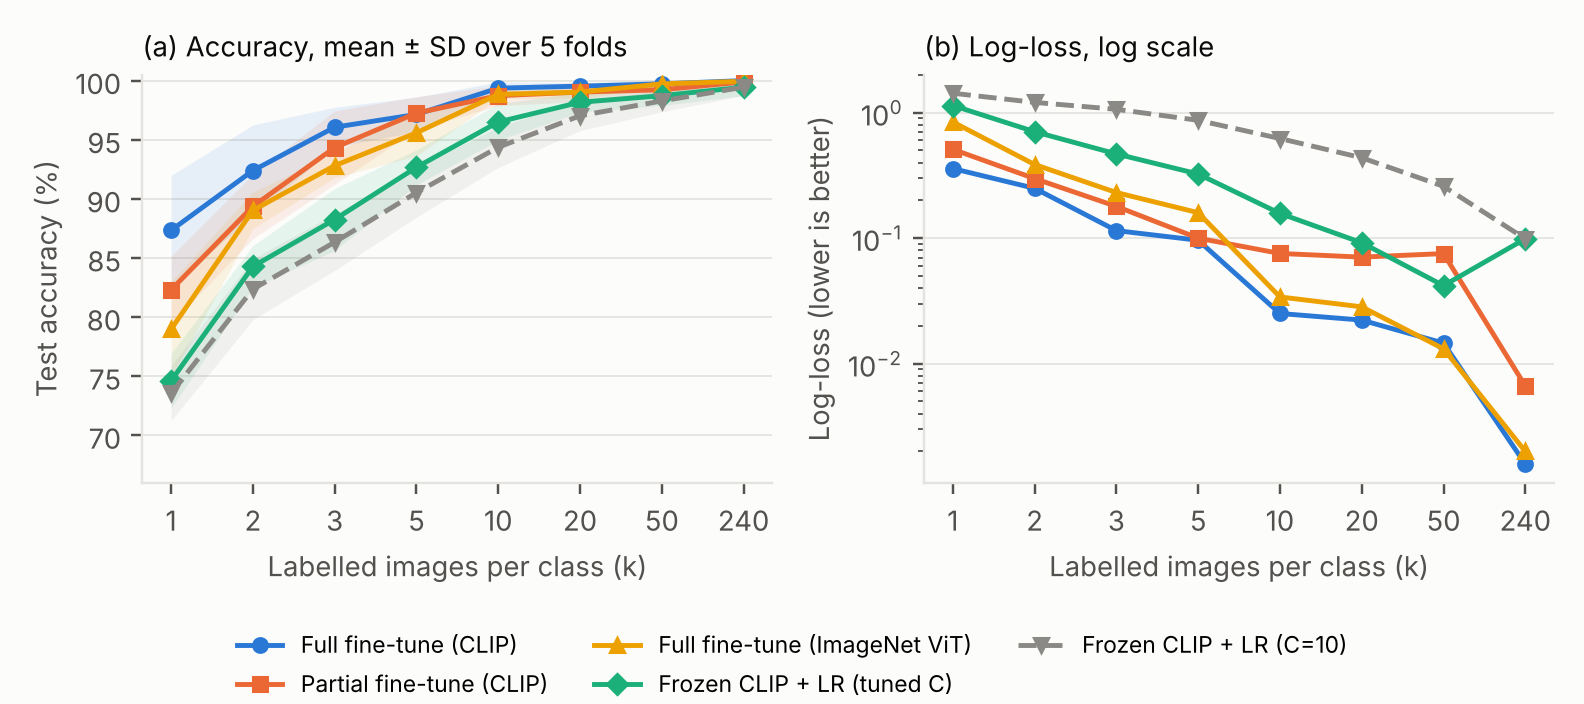
\includegraphics[width=\linewidth]{figures/fig1_learning_curves.png}
\caption{Learning curves (5 folds). (a) Accuracy, shaded $\pm1$ SD over folds. (b) Log-loss.}\label{fig:lc}
\end{figure}

\begin{table}[t]
\centering\small
\caption{Test accuracy (\%), mean $\pm$ SD over 5 folds.}\label{tab:acc}
\begin{tabular}{@{}lcccccc@{}}
\toprule
Labels per class $k$ & 1 & 2 & 5 & 10 & 50 & 240\\
\midrule
Frozen CLIP + LR ($C{=}10$) & 73.6$\pm$2.3 & 82.4$\pm$2.6 & 90.5$\pm$2.1 & 94.4$\pm$1.7 & 98.3$\pm$0.9 & 99.4$\pm$0.7\\
Frozen CLIP + LR (tuned) & 74.6$\pm$2.3 & 84.3$\pm$1.8 & 92.7$\pm$1.5 & 96.5$\pm$1.5 & 98.7$\pm$0.8 & 99.4$\pm$0.7\\
Partial fine-tune (CLIP) & 82.3$\pm$2.9 & 89.4$\pm$2.7 & 97.3$\pm$1.4 & 98.7$\pm$0.8 & 99.2$\pm$0.6 & 99.9$\pm$0.3\\
Full fine-tune (CLIP) & \textbf{87.3$\pm$4.7} & \textbf{92.4$\pm$3.9} & 97.1$\pm$1.5 & \textbf{99.4$\pm$0.5} & \textbf{99.7$\pm$0.3} & \textbf{100.0$\pm$0.0}\\
Full fine-tune (ImageNet ViT) & 79.0$\pm$4.0 & 89.0$\pm$1.6 & 95.6$\pm$2.0 & 98.8$\pm$0.4 & 99.7$\pm$0.3 & 99.9$\pm$0.1\\
\bottomrule
\end{tabular}
\end{table}

\textbf{Calibration and confident errors.} Fine-tuned CLIP is well calibrated (ECE 0.008 at $k=10$; log-loss 0.025), whereas the frozen classifier at $C=10$ is under-confident (ECE 0.38; tuning cuts it to 0.07). However, at $k=1$ the fully fine-tuned model misclassifies 2.8\% of test images with probability $\ge0.9$ (22\% of its errors), and the ImageNet ViT 8.3\% (39\% of its errors). The frozen classifier makes no confident errors because it is rarely confident. Average calibration therefore does not guarantee that a high-confidence prediction can be trusted.

\textbf{Rare defects.} With one labelled example of a rare class (others 50), plain fine-tuning finds 6\% of its test images and frozen features 0\%. Class-weighted fine-tuning finds 69\% (52--85\% depending on the class) at precision 1.0, and balanced-weight frozen features 24\%. With 5 examples plain fine-tuning finds 88\% and weighting adds a further 7 points; at 20 examples all fine-tuned variants exceed 98\% (Fig.~\ref{fig:rare}a).

\textbf{Unseen defects.} Using maximum softmax probability~\cite{hendrycksgimpel}, fine-tuned CLIP separates an unseen defect type from known ones best (AUROC 0.963; false-positive rate at 95\% recall 0.12), ahead of partial fine-tuning (0.925), frozen nearest-neighbour distance (0.876) and frozen logistic regression (0.866; Fig.~\ref{fig:rare}b). The spread across defect types and methods is large (0.78--0.99), so a defect-specific alarm threshold would be needed.

\begin{figure}[t]
\centering
\begin{subfigure}{0.52\linewidth}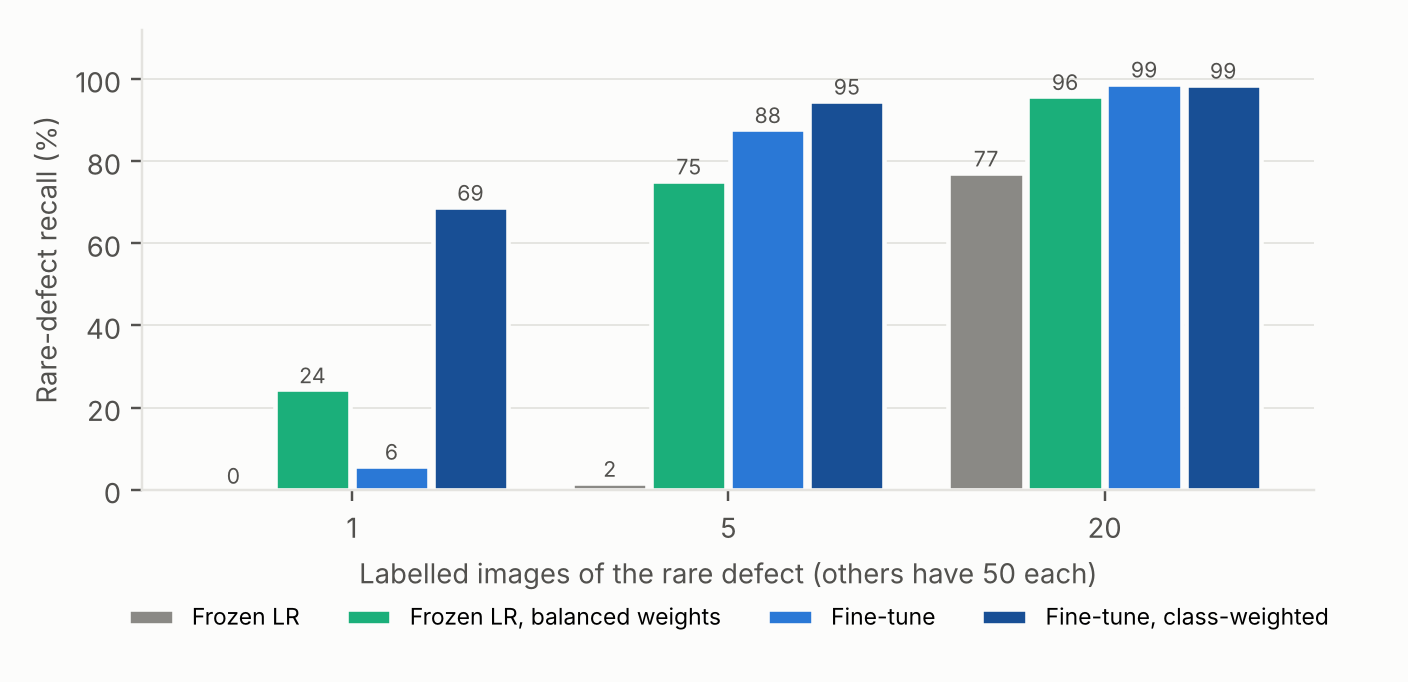
\includegraphics[width=\linewidth]{figures/fig2_rare_defect.png}\caption{Rare-defect recall}\end{subfigure}\hfill
\begin{subfigure}{0.46\linewidth}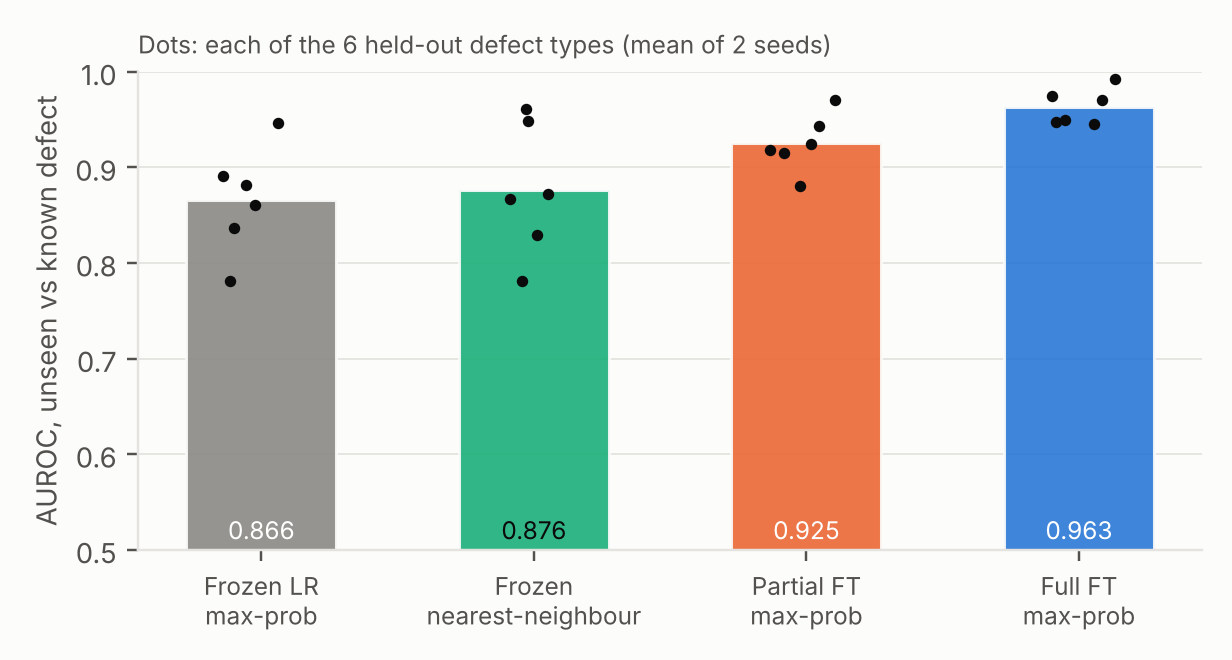
\includegraphics[width=\linewidth]{figures/fig3_open_set.png}\caption{Unseen-defect AUROC}\end{subfigure}
\caption{(a) Recall for a rare class (mean over 3 classes $\times$ 2 seeds). (b) AUROC, dots are the six held-out defects.}\label{fig:rare}
\end{figure}

\textbf{Corruptions.} Models trained on clean images ($k=20$) degrade sharply under blur and noise~\cite{hendrycksdiet} (Fig.~\ref{fig:rob}): at the heaviest blur, accuracy is 61\% (CLIP full), 74\% (ImageNet ViT) and 40\% (frozen); at the heaviest noise, 68\%, 84\% and 38\%. Adding blur and noise augmentation restores 97\% and 96\%. This shows protection against distortions it was trained on, not general robustness: under strong brightening ($\times1.4$) the augmented model is slightly worse (96.4\% versus 98.5\%; 95.6\% versus 99.0\% at $k=240$). These tests use one fold's 360 test images and two seeds.

\begin{figure}[t]
\centering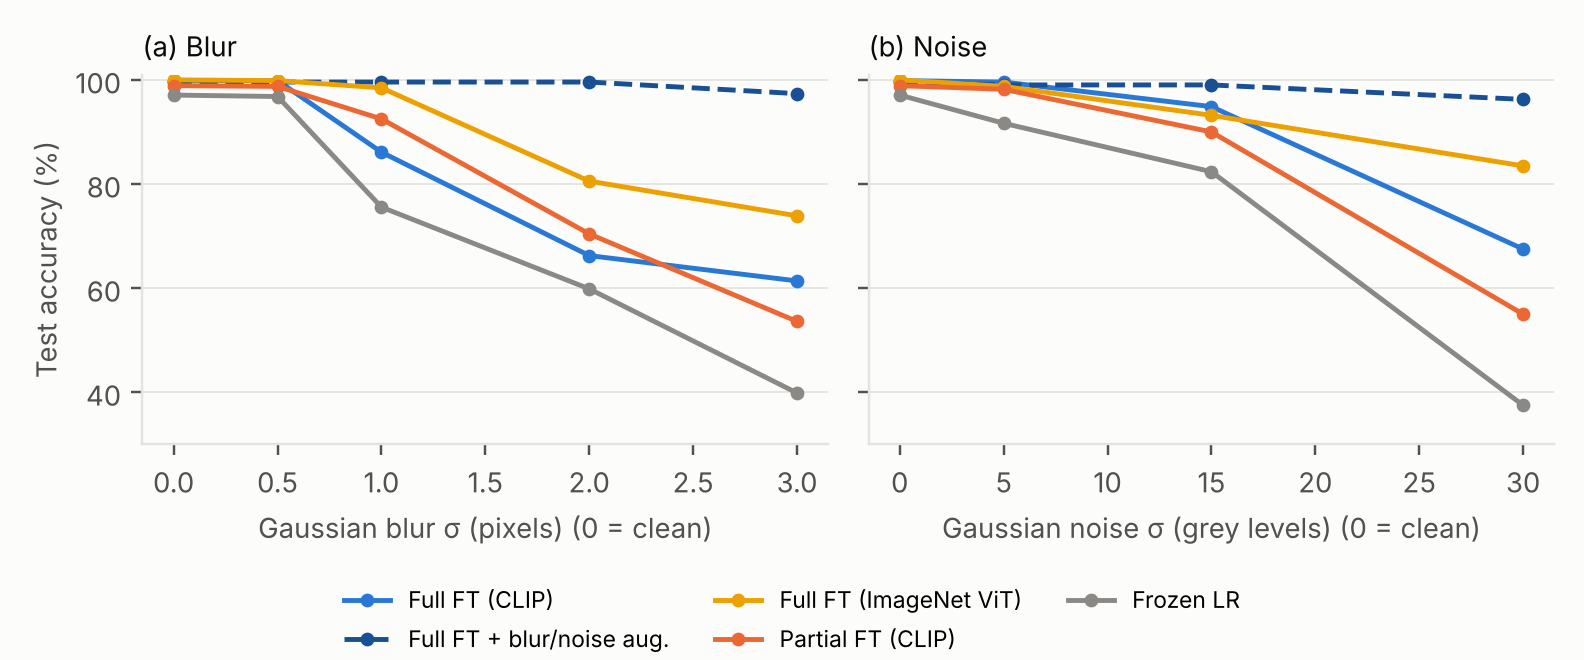
\includegraphics[width=\linewidth]{figures/fig4_robustness.png}
\caption{Accuracy under blur and noise ($k=20$, fold 0, 2 seeds).}\label{fig:rob}
\end{figure}

\textbf{Sensitivity and zero-shot.} Fine-tuned accuracy varies little across three learning rates ($96.0$--$96.9\%$ at $k=5$; $99.0$--$99.4\%$ at $k=20$), while the frozen classifier is very sensitive to regularisation (91.2\% to 98.5\% across the four values at $k=20$). Zero-shot CLIP, with prompts chosen on the training pool, scores 19.7\% against 16.7\% for guessing, with half of all predictions assigned to ``patches''; the text encoder has no useful vocabulary for these defects, although its image features do.

\textbf{Qualitative checks.} Occlusion maps (Fig.~\ref{fig:occ}) are one image per class and scaled per panel, so they only indicate that models rely on different regions: for the inclusion example the frozen model gives the true class probability 0.20 and the fine-tuned model 0.97. We make no causal claims from them.

\textbf{Limitations of the evidence.} Saturation above 50 labels, a single homogeneous dataset, 360 test images per fold, non-independent folds, and one fold only for the corruption and sensitivity tests limit generality. We include no convolutional baseline, so claims concern ViTs only.

\begin{figure}[t]
\centering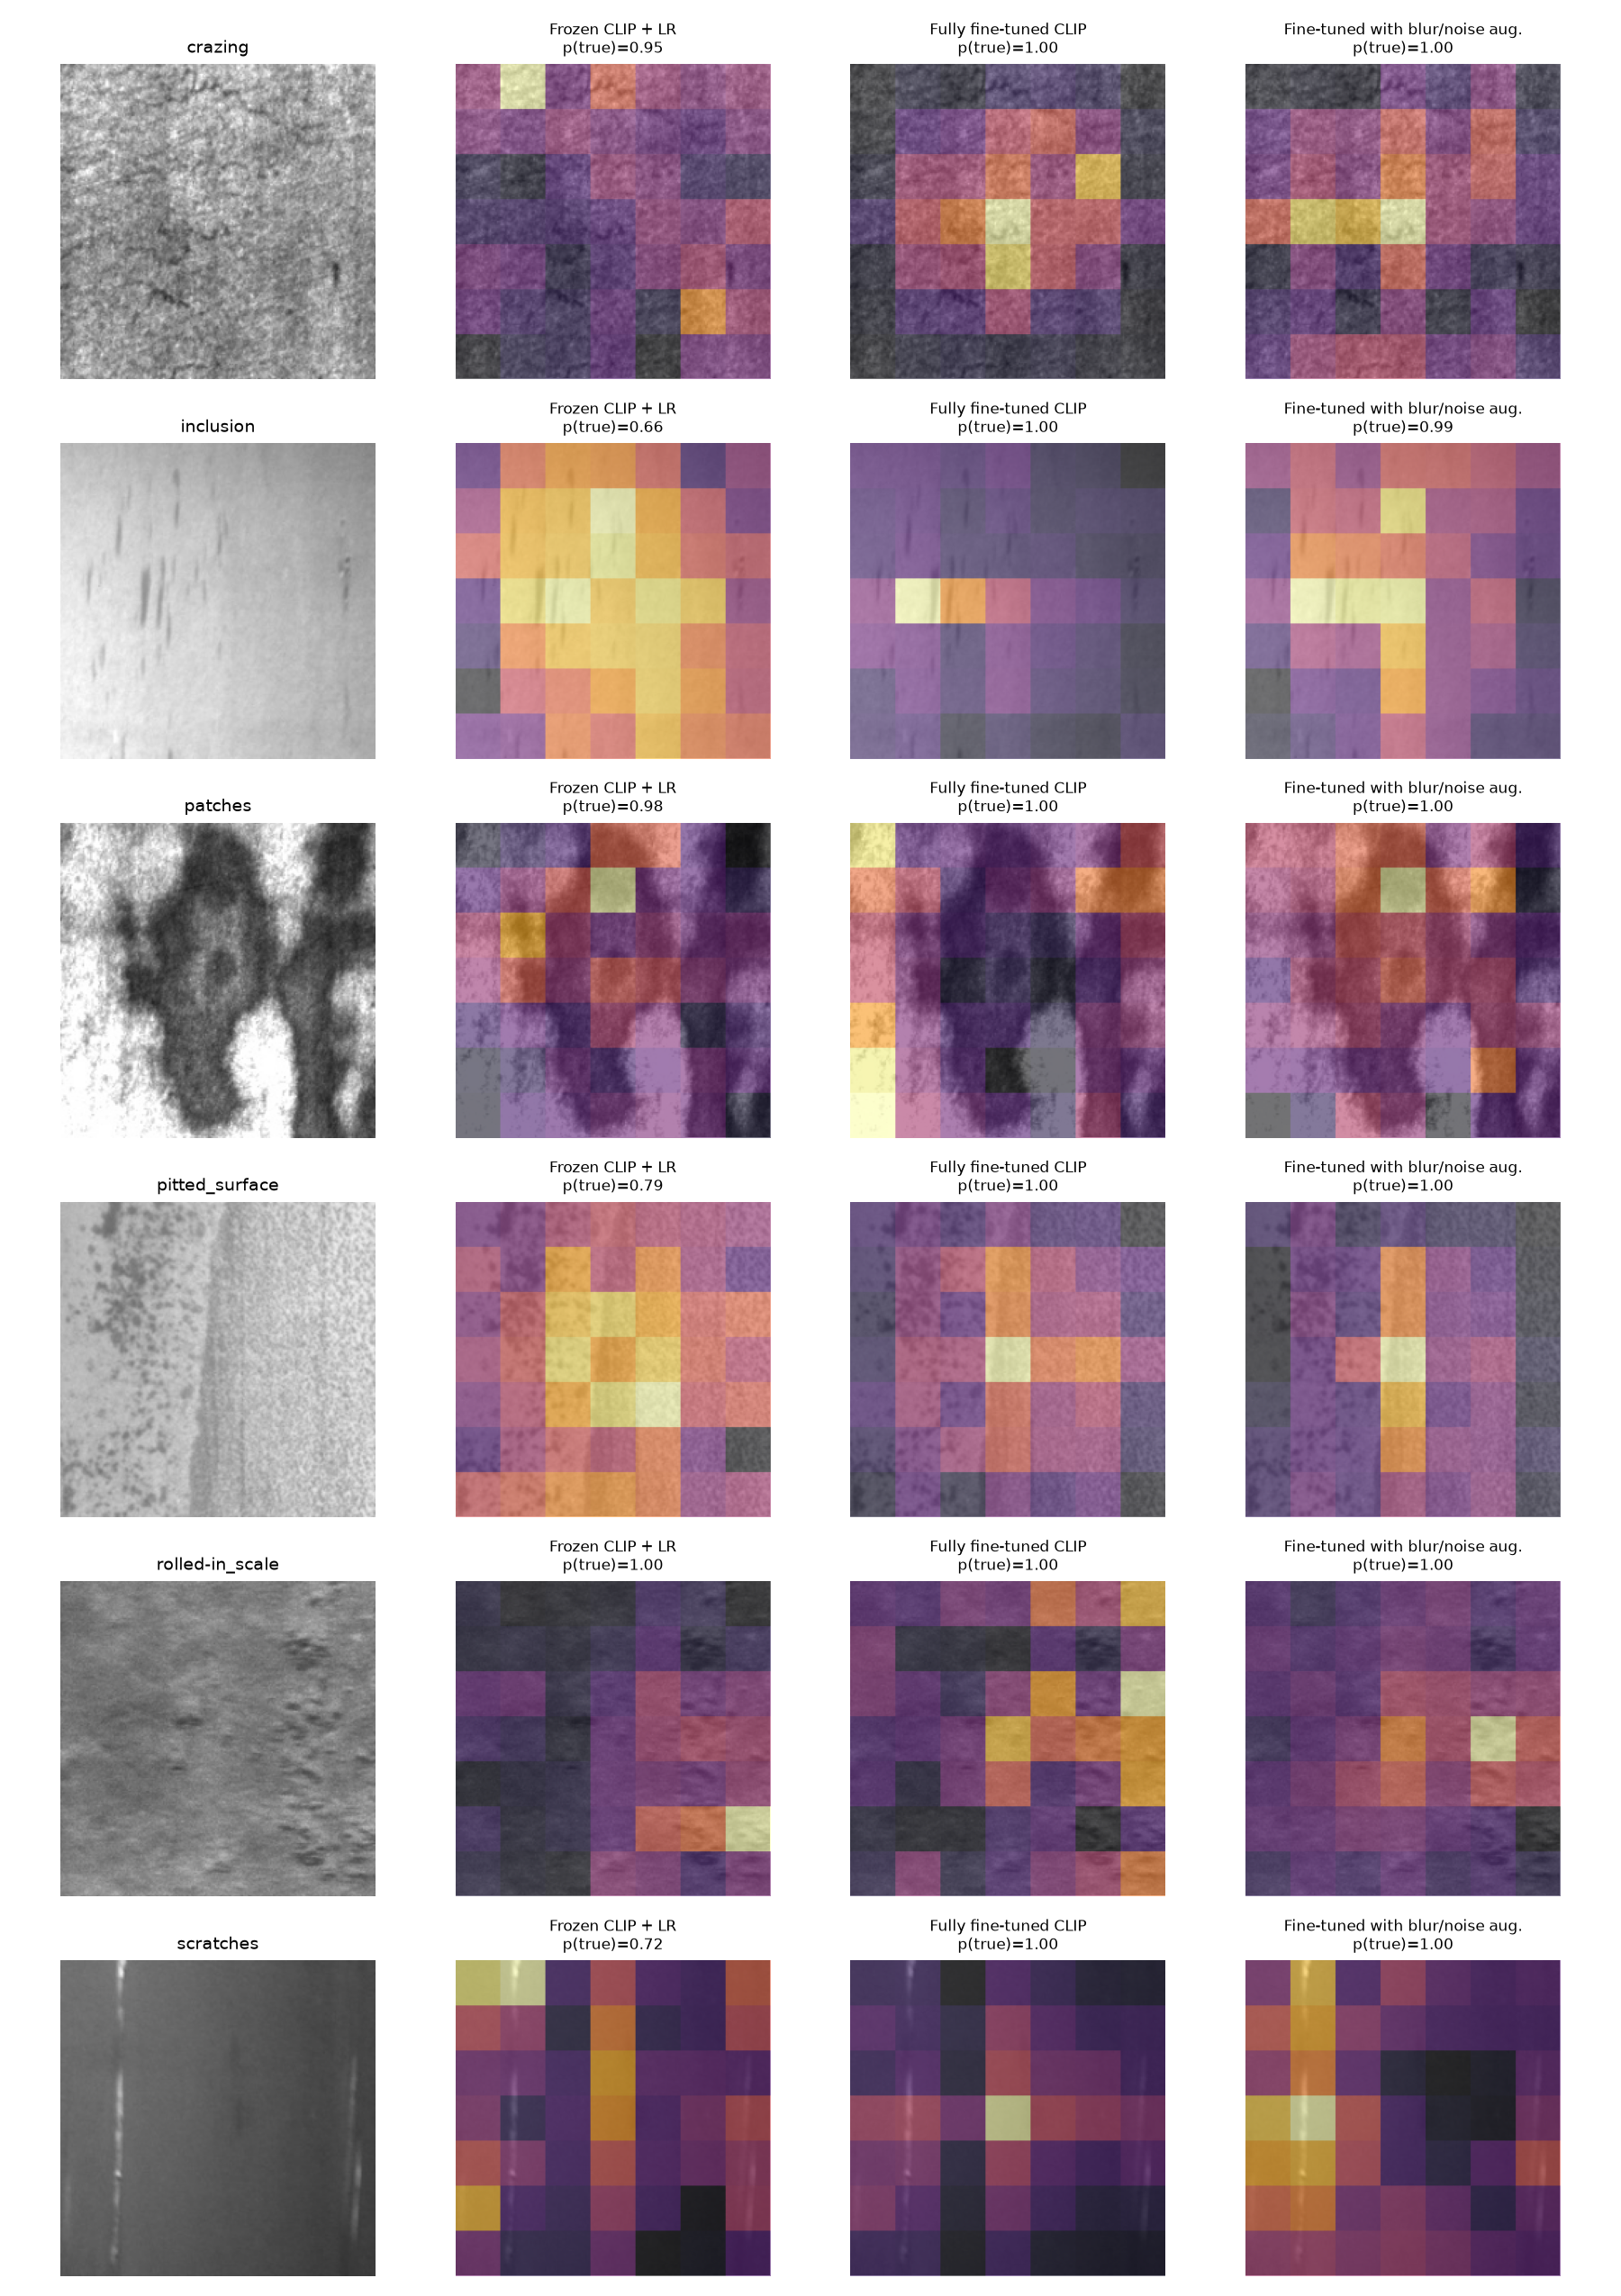
\includegraphics[width=0.5\linewidth]{figures/occlusion_maps.png}
\caption{Occlusion sensitivity: brighter areas lower the true-class probability more when hidden.}\label{fig:occ}
\end{figure}

\begin{figure}[t]
\centering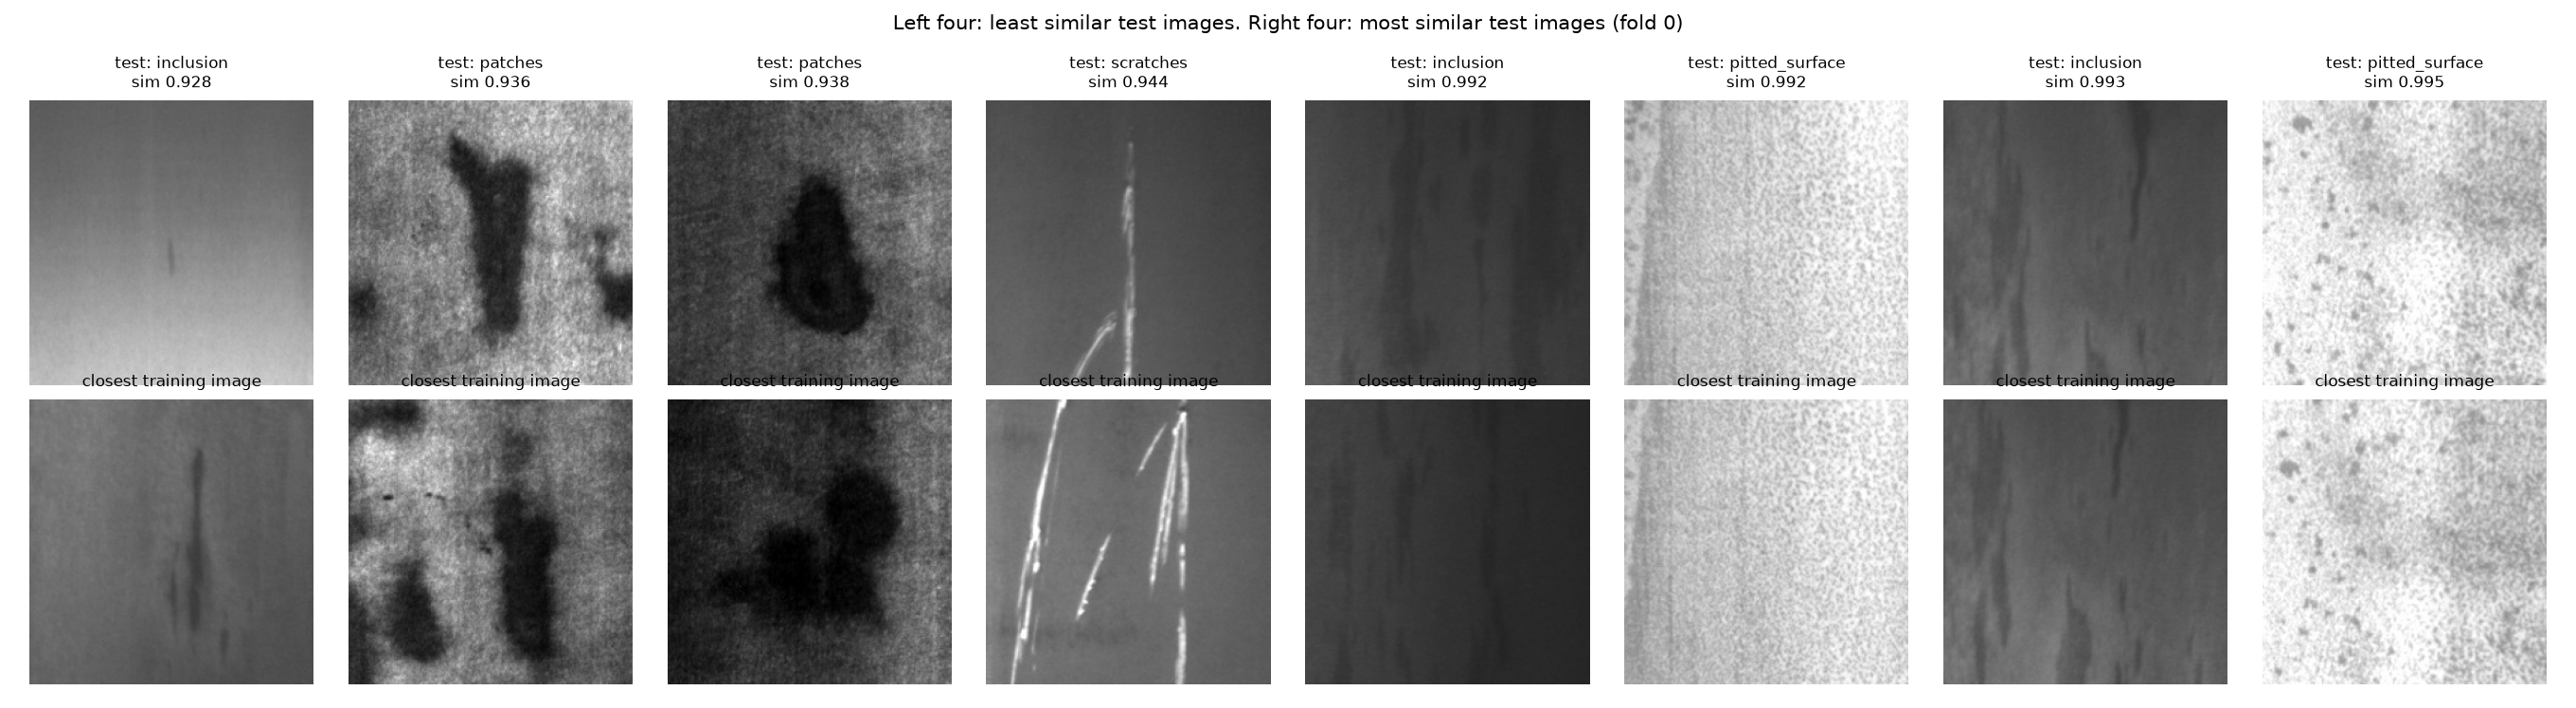
\includegraphics[width=\linewidth]{figures/nearest_training_images.png}
\caption{Least similar (left four) and most similar (right four) test images with their closest training image.}\label{fig:nn}
\end{figure}

\section{Ethical and Societal Considerations}
\textbf{Safety and accountability.} A missed defect can ship a faulty product, and a false alarm wastes steel. Our confident-error result means a high softmax score cannot by itself authorise automatic release; we recommend human review of low-confidence and novel-looking items, a calibrated threshold per defect type, and logging every decision. Responsibility for missed defects must stay with the plant's quality function, not the model, in line with the accountability and transparency that Dubai's AI ethics toolkit asks organisations to prioritise~\cite{dubaiai}.

\textbf{Data, bias and provenance.} NEU contains images of steel only; no people appear, so personal-data rules such as the UAE federal data protection law~\cite{pdpl} are not engaged. Deploying cameras on a shop floor could change that, and would require lawful processing and data minimisation. CLIP was pretrained on web-scale image--text data whose contents we could not audit~\cite{clip}; bias there is unlikely to matter for steel textures, but we did not measure it. The more relevant bias is dataset bias: one laboratory setup and homogeneous images mean reported accuracy may not transfer to other plants, camera positions or steel grades; models should be revalidated on local data. We recommend documenting the data and models with datasheets and model cards~\cite{datasheets,modelcards}; the repository includes a short model card.

\textbf{Workforce.} The UAE AI strategy lists manufacturing among sectors with high automation potential and stresses training for new jobs~\cite{uaeai}. A model like ours should assist inspectors, who handle low-confidence and novel cases, rather than replace them; because a few labels give useful accuracy, staff can help label and audit local data, building skills rather than only displacing them.

\textbf{Environment and transparency.} Fine-tuning costs far more compute than extracting frozen features, a footprint that grows with experiment count~\cite{strubell}. Our suite was run on a laptop; we did not measure energy, and our own choice to run many repeated experiments is part of that cost. We therefore recommend frozen features when labels are plentiful, since they perform within about one point of fine-tuning. Finally, we report all prompt and parameter variants, including the weak zero-shot result, rather than only favourable settings.

\section{Conclusion and Future Work}
When labels are very scarce (1 to 5 per class), fully fine-tuning a CLIP ViT is clearly better than a frozen encoder, reaching 95\% with 3 labels per class, and class-weighted fine-tuning is the best of the methods tested for rare defects. With 50 or more labels, a tuned frozen encoder is nearly as good at a fraction of the cost. Fine-tuned models are well calibrated on average yet still make confident mistakes, and robustness to blur and noise needs specific training. Limitations include a homogeneous single dataset and few folds for some tests. Future work: a second, more varied dataset (for example GC10-DET or X-SDD); detection rather than classification; parameter-efficient or weight-averaged fine-tuning to protect pretrained features~\cite{kumar}; calibrated or conformal abstention; and testing under a camera or plant shift.

\bibliographystyle{ieeetr}
\bibliography{refs}

\end{document}
